\documentclass[conference]{IEEEtran}
\usepackage[T1]{fontenc}
\usepackage[utf8]{inputenc}

%\usepackage{fullpage}
\usepackage[french, english]{babel}
\usepackage{amsmath,amsfonts,amssymb}
\usepackage{graphicx, tikz}
\usepackage{todonotes}
\usetikzlibrary{shapes,snakes}
\usetikzlibrary{arrows}
\usetikzlibrary{positioning}

\definecolor{mygreen}{rgb}{0.55, 0.71, 0.0}
\usepackage{mathtools}
\usepackage{xcolor}
\usepackage{rotating}
\usepackage{lipsum}
\usepackage{caption}
\usepackage[backend=biber]{biblatex}
\bibliography{Biblio}{}


\newenvironment{keywords}%
{\description\item[Mots-clés.]}%
{\enddescription}

\title{DeepVoice}

\author{Rémi Hutin, Rémy Sun, Raphaël Truffet \\
  \{Remi.Hutin, Remy.Sun, Raphael.Truffet\}@ens-rennes.fr \\
  Département informatique, ENS Rennes \\
  Campus de Ker lann, Bruz, France
\and
  Guillaume Gravier, Vedran Vukotić\\
  \{guig, vedran.vukotic\}@irisa.fr\\
  Linkmedia project, IRISA \\
  Campus de Beaulieu, Rennes, France
}

\begin{document}

\maketitle

\begin{abstract}
  To carry out a speaker recognition task, i.e., to identify the speaker in an
audio signal, one must first obtain a serviceable representation
of said signal. Improvements upon the raw numeric signal have been made over the
years, one of which is the creation of a Gaussian mixture model supervector
representing the probabilistic distribution of the signal's
spectral features. Due to the enormous size of such supervectors, condensed
forms such as i-vectors have been created to provide usable data for application
tasks. Deep learning techniques have seen significant success in many
classification tasks due to their ability to
build upon successive layers of data representation. We will
strive to explore the possibility of using such techniques to acquire a
representation of supervectors that is at least competitive with i-vectors.

\end{abstract}
\begin{IEEEkeywords}
  Speaker recognition; Deep learning;  i-vector; Latent representation
\end{IEEEkeywords}
\section{Introduction}

Speaker recognition refers to the all too important identification of a speaker
from an unlabeled audio signal. However, the resolution of this essential issue
is no trivial matter as it raises a number of questions along the way. The most
immediate one, is the manner in which the data will be represented: raw numeric
signal, Fourier transform, spectral representation?

Years of research into the issue have yielded a solution called
\emph{supervectors} which provide a probabilistic representation of the
numeric signal's spectral features. Those supervectors however present the
significant downside of being enormous and containing information not relevant
to the task at hand, which makes them unfit for applications. What recent works
have had success with is the extraction of more condensed representations from
those supervectors named \emph{i-vectors}.

Deep learning techniques have had tremendous success in a number of fields
ranging from computer vision \cite{lecun1998gradient} to natural language
processing \cite{bordes2012joint} by building upon successive layers of data
representation and inferring hierarchical dependencies within the data. It seems
to us that such architectures would be especially adapted to the extraction of
intermediate representations from \emph{supervectors} and might provide
representations that outperform the current state of the art \emph{i-vectors}.

To begin with, we will give a brief exposition of signal representations used
up until now \ref{sec:signal}. Afterwards, a brief explanation of the Deep
Learning techniques we will need will be provided \ref{sec:Deep}. Finally, we
will give an overview of the study we plan to conduct \ref{sec:Method}

\section{Sound signals}
\label{sec:signal}
An audio signal used for speaker recognition tasks is technically an analogical
signal. To allow computer processing, those signals are sampled into a numeric
signal (discrete set of measures that can a discrete set of values). Such a
representation is highly vulnerable to noise and transformations however,
and more developed means of representation are usually used.

\subsection{Cepstral analysis}

The speech signal of a speaker is hardly suitable for statistical modeling or
the calculation of a distance.
In order to obtain a representation which is more compact and less redundant, we
use a cepstral representation of the speech.
The cepstrum of a signal $x(t)$ is defined by \eqref{eq:cepstrum}

\begin{equation}
  C(x(t)) = \mathcal{F}^{-1}(\ln(|\mathcal{F}(x(t))|)
   \label{eq:cepstrum}
\end{equation}

where $\mathcal{F}$ is the Fourier transform.
We can analyze a signal locally by applying a short-term window. Then, we
extract a vector of cepstral coefficients of this part of signal. We repeat
this operation for several windows, until the end of the signal is reached.

In the cepstral domain, the distance between two speech signals may be easily
computed using the Euclidean distance.


\subsection{Gaussian mixture model (GMM) and supervectors}

A Gaussian mixture model (GMM) is a probabilistic model used to approximate a
distribution of random variables as a sum of normal distributions (\cite{Bimbot2004}).
Here, we suppose that cepstral vectors of a signal follow a probability
distribution that is specific to the given signal. This distribution is the one
that we try to approximate with the GMM using a reference model. In fact, even
if the distribution is specific to the given signal, the form of the
distribution is universal for the natural language and called the Universal
Background Model (UBM). The supervector is the vector that gather means of
all the normal distributions of the GMM. Such models are used to represent
signals in speaker recognition tasks (Figure \ref{gmm})\\


\begin{figure}[!h]
    \centering
    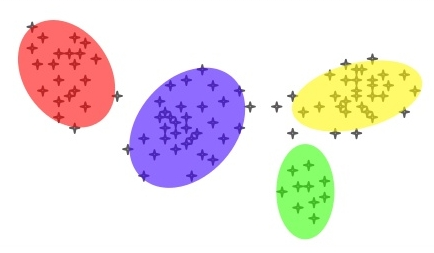
\includegraphics[width=7cm]{GMM.jpg}
    \caption{Gaussian Mixture Model with 4 Gaussian distributions (GMM)}
    \label{gmm}
\end{figure}

\subsection{I-vectors}

A supervector presents a probabilistic representation of a signal's spectral features.
However, these supervectors are enormous, which makes them unfit for
applications and, since they contain information on the entire signal, contain
information of little interest to us.
That's why we want a more condensed version a these supervectors.


Let $M$ be the supervector, obtained as explained previously. $M$ depends on the speaker and on the channel.
We will perform a \emph{linear projection}, to express $M$ as

\begin{equation}
  M = m + Tw
  \label{eq:i}
\end{equation}

\noindent where
\begin{itemize}
\item $m$ is a speaker and channel independent supervector
\item $T$ is a rectangular matrix, called \emph{Total-variability matrix}
\item $w$ is an intermediate vector, or \emph{i-vector}
\end{itemize}

The typical size of $w$ is $60$. These linearly extracted \emph{i-vectors} provide lighter, and therefore more usable, data for application tasks.

\subsection{Previous works}


Extracting the i-vector is interesting for speaker recognition because it is
easier to apply usual classifications method on it as cosine distance scoring
(CDS) and support vector machines (SVM) \cite{Senoussaoui_ani-vector,
  dehak2011front}. I-vectors are good tools for speaker recognition because they
are channel independent and compact. We will try to keep these two
characteristics in the new representation we will build using neural networks.




\section{Use of neural networks}
\label{sec:Deep}
The recent success of deep learning techniques in various fields such as
computer vision \cite{lecun1998gradient} and natural language processing \cite{bordes2012joint} has sparked
many explorations of their usefulness in classification tasks on
\emph{i-vectors} such as speaker recognition. Many architectures such as deep
belief networks \cite{DBLP:journals/corr/GhahabiH15},\cite{ghahabi2014deep},
deep neural networks \cite{DBLP:journals/corr/GhahabiH15},\cite{ghahabi2014deep}, recurrent
networks \cite{DBLP:journals/corr/SaonSRK16} or even a mix of
deep neural networks and support vector machines \cite{richardson2015deep} have been tested and yielded
better results than previous techniques, though -- to the best of our knowledge --
none directly tackled the issue of supervectors' intermediate representation.
Instead, all of the aforementioned work relied on pre-existing i-vector
extraction techniques. We will explore the possibility of extracting a
meaningful intermediate representation of supervectors through the use of deep architectures.

\subsection{Formal neuron}

\def\layersep{2cm}

\begin{figure}[!tbp]

\centering
\begin{tikzpicture}[shorten >=1pt,->,draw=black!50, node distance=\layersep]
    \tikzstyle{every pin edge}=[<-,shorten <=1pt]
    \tikzstyle{neuron}=[ellipse,fill=black!25,minimum size=17pt,inner sep=0pt]
    \tikzstyle{input neuron}=[neuron, fill=green!50];
    \tikzstyle{output neuron}=[neuron, fill=red!50];
    \tikzstyle{hidden neuron}=[neuron, fill=blue!50];
    \tikzstyle{hidden neuron back}=[neuron, fill=orange!50];
    \tikzstyle{annot} = [text width=8em, text centered]

    % Draw the input layer nodes
    \foreach \name / \y in {1,...,4}
    % This is the same as writing \foreach \name / \y in {1/1,2/2,3/3,4/4}
        \node[input neuron, pin=left:] (I-\name) at (0,-\y) {$a_\y$};

    % Draw the hidden layer nodes
    \foreach \name / \y in {1,...,1}
        {
        \path[yshift=-1.5cm]
        node[hidden neuron] (H-\name) at (\layersep,-\y cm) {};
        }

    % Draw the output layer node
    \node[output neuron, right =1cm of H-1] (O) {\footnotesize$e = f(WA + b)$};

    % Connect every node in the input layer with every node in the
    % hidden layer.
    \foreach \source in {1,...,4}
        \foreach \dest in {1,...,1}
            \path (I-\source) edge (H-\dest);

    % Connect every node in the hidden layer with the output layer
    \foreach \source in {1,...,1}
        \path (H-\source) edge (O);

    % Annotate the layers
    \node[annot,below of=H-1, node distance=1cm] (wb) {Weight $W$\\Bias $b$};
    \node[annot,above of=H-1, node distance=1cm] (n) {Neuron};
    \node[annot,above of=I-1, node distance=1cm] (ia) {Input A};

\end{tikzpicture}

    \caption{Formal neuron}
    \label{fig:neur}
\end{figure}
\def\layersep{1.5cm}
\begin{figure}[!tbp]
\begin{tikzpicture}[shorten >=1pt,->,draw=black!50, node distance=\layersep]
    \tikzstyle{every pin edge}=[<-,shorten <=1pt]
    \tikzstyle{neuron}=[circle,fill=black!25,minimum size=17pt,inner sep=0pt]
    \tikzstyle{input neuron}=[neuron, fill=green!50];
    \tikzstyle{output neuron}=[neuron, fill=red!50];
    \tikzstyle{hidden neuron}=[neuron, fill=blue!50];
    \tikzstyle{hidden neuron back}=[neuron, fill=orange!50];
    \tikzstyle{annot} = [text width=4em, text centered]

    % Draw the input layer nodes
    \foreach \name / \y in {1,...,4}
    % This is the same as writing \foreach \name / \y in {1/1,2/2,3/3,4/4}
        \node[input neuron, pin=left:] (I-\name) at (0,-\y) {$a_\y$};

    % Draw the hidden layer nodes
    \foreach \name / \y in {1,...,5}
        {
        \path[yshift=0.5cm]
        node[hidden neuron] (H1-\name) at (\layersep,-\y cm) {};
        }

    \foreach \name / \y in {1,...,4}
        {
        \path
        node[hidden neuron] (H2-\name) at (2*\layersep,-\y cm) {};
        }

    \foreach \name / \y in {1,...,5}
        {
        \path[yshift=0.5cm]
        node[hidden neuron] (H3-\name) at (3*\layersep,-\y cm) {};
        }
    % Draw the output layer node
    \node[output neuron,pin={[pin edge={->}]right:Output}, right of=H3-3] (O) {};

    % Connect every node in the input layer with every node in the
    % hidden layer.

    \foreach \source in {1,...,4}
        \foreach \dest in {1,...,5}
            \path (I-\source) edge (H1-\dest);



    \foreach \source in {1,...,5}
        \foreach \dest in {1,...,4}
            \path (H1-\source) edge (H2-\dest);


    \foreach \source in {1,...,4}
        \foreach \dest in {1,...,5}
            \path (H2-\source) edge (H3-\dest);


    \foreach \source in {1,...,5}
        \path (H3-\source) edge (O);



    % Annotate the layers
    \node[annot,above of=H1-1, node distance=1cm] (hl1) {Hidden layer 1};
    \node[annot,right of=hl1] (hl2) {Hidden layer 2};
    \node[annot,right of=hl2] (hl3) {Hidden layer 3};
    \node[annot,right of=hl3] {Output layer};
    \node[annot,left of=hl1] {Input layer};

    \node[annot,below of=H1-5, node distance=1cm] (wb1) {$W_1$, $b_1$};
    \node[annot,right of=wb1] (wb2) {$W_2$, $b_2$};
    \node[annot,right of=wb2] (wb3) {$W_3$, $b_3$};
\end{tikzpicture}

    \caption{Deep neural network}
    \label{fig:net}
\end{figure}


\paragraph{Neuron}

Neural networks can be fairly complicated to understand all at once, and
therefore we will start by explaining how one of its basic units work.
A neuron (Figure \ref{fig:neur}) can be thought of as a function which takes an $n$-dimensional vector
$A$ as input and returns a scalar $e$ as output. This function typically has two
internal parameters which are a bias $b$ and a weight matrix $W$. The function
starts by calculating $WA+b$ before using a non-linear activation function (such
as sigmoid or tanh), i.e.,

\begin{equation}
  e=f(WA+b).
\end{equation}

\paragraph{Adjusting the function}

Our end goal is to have the neuron, and by extension the neural network (which we
will introduce later), perform
a certain task. The formal neuron \og learns\fg{} by adjusting its function to perform better on
a designated task. For simplicity's sake, we will first explain how a
process -- called \og back-propagation\fg{} -- works with a single neuron.

For instance, suppose we have a bi-dimensional vector given as input and that we
want our neuron to return 1 if its two coordinates are the identical and -1 if
they are not. A natural way to evaluate how accurate our neuron consists in looking at the
distance between its output $e$ and the desired result r :

\begin{equation}
d(e)=|e-r|
\end{equation}

\noindent We want to modify our neuron/function to minimize this distance. That means
changing $e$, typically by gradient descent on function $d$ derivative. Here,
$\frac{\partial d}{\partial e} = r-e$, which means we want to \og move\fg{} $e$ in this
direction. To this end, we modify our function's two internal parameters $W$ and
$b$. $e$, and by extension $d$, can actually be seen as a function of those two
parameters: $d(W,b)=|e(W,b)-r|$. Therefore $\frac{\partial d}{\partial W}
   = \frac{\partial d}{\partial e}\frac{\partial e}{\partial W}$,
$\frac{\partial d}{\partial b}
   = \frac{\partial d}{\partial e}\frac{\partial e}{\partial b}$. We then only
   need to compute new internal parameters $W'$ and $b'$ with \ref{eq:W} and \ref{eq:b}.

\begin{equation}
  W'=W + s\frac{\partial d}{\partial W}=W-s\frac{\partial d}{\partial e}\frac{\partial e}{\partial W}
  \label{eq:W}
\end{equation}

\begin{equation}
  b'=b + s\frac{\partial d}{\partial b}=b-s\frac{\partial d}{\partial e}\frac{\partial e}{\partial b}
  \label{eq:b}
\end{equation}

What we just demonstrated was a simple back-propagation algorithm called gradient
descent. This method is deeply flawed, but most state of the art back-propagation
methods find their origins in this humble algorithm.

\paragraph{Neural network}

Typically, a neural \textbf{network} (Figure \ref{fig:net}) is made up of more than a single neuron. A
neural layer refers to multiple neurons working on the same input (or parts of
the same input) and producing an output that can be construed as some form of
concatenation of their respective outputs. This output can be in turn regarded
as an alternate representation of the input. Back-propagation for each neuron
works the same way as it would if it were the only neuron calculating.

The notion of \textbf{deep} learning comes from the fact that the alternate
representation computed by one layer $A$ can be fed as input to another layer $B$.
This allows networks to infer multiple levels of representation, same as one
first processes simple geometrical forms before recognizing more complex
compositions. Back-propagation is straight-forwardly computed on layer $B$. It is
computed on layer $A$ by looking at $\frac{\partial d}{\partial input_B}$
instead of $\frac{\partial d}{\partial e}$ which is simply calculated using the
rule of chain derivation:

\begin{equation}
  \frac{\partial f}{\partial x}=\frac{\partial f}{\partial x_1}...\frac{\partial x_k}{\partial x}.
\end{equation}

What is of particular interest to us is the intermediate representations the
network acquires this way. Indeed, our goal is to obtain a representation of
supervectors that outperforms the linear extraction of i-vectors.

\subsection{Autoencoders}

An autoencoder \cite{Hinton504} is a neural network with a particular
architecture which is defined below.

\paragraph{A default task for a different goal}

Neural networks' ability to extract internal meaningful representation from the
original raw data is very enticing. Indeed, providing a meaningful
representation of the initial data is one of the biggest hurdles of classical
machine learning. However, neural networks need to be trained on a task, and
require labeled data to that end.

Since we are no longer interested in the specific task needed to train the
network, it is possible to default to a task that is not interesting in itself
but might require the network to learn salient features of the data in order to
be completed. A very natural one is to match the output to the input, which
would not require man made labeling. Hopefully, the learned representation will
capture features specific to the input so that it may be reconstructed.

\paragraph{Structure}

Typically, the \textbf{input} is \textit{encoded} \eqref{eq:enc} into a \textbf{latent
  representation} which is then \textit{decoded} \eqref{eq:dec} into an \textbf{output} that
should match the input as closely as possible, hence the autoencoder
denomination (Figure \ref{autoencoder_structure}). The main danger of such an approach is having the networks that
does not transform the input at all and yields a latent representation that is
no different to the raw input data. A multitude of solutions exist to avoid such
a scenario:
\begin{itemize}
\item Compress the input into a latent representation of lower dimension
\item Put the input through a corrupting input layer: the autoencoder cannot
  just do nothing and give back the same thing because it never had the actual
  input to begin with. This particular structure is called denoising auto-encoder.
\item Use various regularization methods.
\end{itemize}

\begin{figure}[!h]
    \centering

\begin{tikzpicture}[yscale=0.7, shorten >=1pt,->,draw=black!50, node distance=\layersep]
    \tikzstyle{every pin edge}=[<-,shorten <=1pt]
    \tikzstyle{neuron}=[circle,fill=black!25,minimum size=17pt,inner sep=0pt]
    \tikzstyle{input neuron}=[neuron, fill=green!50];
    \tikzstyle{output neuron}=[neuron, fill=red!50];
    \tikzstyle{hidden neuron}=[neuron, fill=blue!50];
    \tikzstyle{hidden neuron back}=[neuron, fill=orange!50];
    \tikzstyle{annot} = [text width=10em, text centered]

    \path [draw, thick] (-1.2,0.5) rectangle (3.7,-5.6);
    \path [draw, thick] (2.3,0.3) rectangle (7,-5.8);


    % Draw the input layer nodes
    \foreach \name / \y in {1,...,5}
    % This is the same as writing \foreach \name / \y in {1/1,2/2,3/3,4/4}
    	{
        	\node[input neuron, pin=left:] (I-\name) at (0,-\y) {};
		}
    % Draw the hidden layer nodes
    \foreach \name / \y in {1,...,4}
        {
        	\path[yshift=-0.5cm]
            node[hidden neuron] (H1-\name) at (\layersep,-\y cm) {};
        }

    \foreach \name / \y in {1,...,5}
        {
            \path
            node[hidden neuron] (H2-\name) at (2*\layersep,-\y cm) {};

        }

    \foreach \name / \y in {1,...,4}
        {
        	\path[yshift=-0.5cm]
            node[hidden neuron] (H3-\name) at (3*\layersep,-\y cm) {};
        }

    % Draw the output layer nodes
    \foreach \name / \y in {1,...,5}
        {
        	\path
            node[output neuron,pin={[pin edge={->}]right:}] (H4-\name) at (4*\layersep,-\y cm) {};
        }

    % Connect every node in the input layer with every node in the
    % hidden layer.


    \foreach \source in {1,...,5}
        \foreach \dest in {1,...,4}
            \path (I-\source) edge (H1-\dest);



    \foreach \source in {1,...,4}
        \foreach \dest in {1,...,5}
            \path (H1-\source) edge (H2-\dest);


    \foreach \source in {1,...,5}
        \foreach \dest in {1,...,4}
            \path (H2-\source) edge (H3-\dest);

    \foreach \source in {1,...,4}
        \foreach \dest in {1,...,5}
            \path (H3-\source) edge (H4-\dest);

    \node[annot,above of=I-1, node distance=0.7cm] (xi) {$x_{input}$};
    \node[annot,above of=H2-1, node distance=0.7cm] (xl) {$x_{latent}$};
    \node[annot,above of=H4-1, node distance=0.7cm] (xo) {$x_{output}$};
    \node[annot,above of=H1-1, node distance=1.8cm] (xl) {encoder};
    \node[annot,above of=H3-1, node distance=1.8cm] (xo) {decoder};





\end{tikzpicture}


    \caption{Structure of an autoencoder}
    \label{autoencoder_structure}
\end{figure}


\begin{equation}
  x_{latent} = encoder(x_{input})
  \label{eq:enc}
\end{equation}

\begin{equation}
  x_{output} = decoder(x_{latent}) \simeq x_{input}
  \label{eq:dec}
\end{equation}


\paragraph{Why use autoencoders}

Autoencoders can be used for denoising, using corrupted data as input and the original data as objective.
Autoencoders may also be very useful to learn a representation. In fact, the latent representation contains enough information to reconstruct the data.

In our context, autoencoders could be used to find a representation of a speaker, by giving to the autoencoder a supervector from a speaker as input, and an another supervector from the same speaker as objective. This idea is based on considering the within-speaker variability as a noise, and using a denoising autoencoder. Repeating this with several pairs of supervectors, we may learn a representation of the speaker. This new representation, as well as i-vectors, is more condensed than supervectors.

Since the problem is symmetrical, we can perform the learning in both directions. One way to perform this training is to use an autoencoder that reconstruct each supervector from the other using tied weights.

\subsection{Tied weight autoencoder}


We talk about tied weight autoencoder when the same weights appears in two
different places in the autoencoder. For example, in the architecture proposed
in \cite{vukotic:hal-01314302}, the weights in light blue in the upper part of the
autoencoder are the same as the weights in light blue in the lower part. So, if
the function that transform the upper first hidden layer to the upper part of
the representation is
\begin{equation}
 h_1(x) = f(W \times x + b_1)
\end{equation}
then  the function that transform the lower part of the representation to the
next layer is
\begin{equation}
 h_2(x) = f(W^T \times x + b_2)
\end{equation}
In this architecture (see Figure \ref{archi_vedran}), the pink weights are also tied.

\begin{figure}[!h]
    \centering
    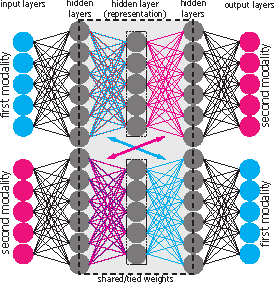
\includegraphics[width=5cm]{archi-vedran.pdf}
    \caption{Symmetrical and bidirectional learning architecture using tied weights}
    \label{archi_vedran}
\end{figure}

This architecture learns a joint representation of the two modalities which gives encouraging results multi-modal query expansion \cite{vukotic:hal-01314302}. In our context, the two modalities will be two supervectors from the same speaker.

\section{Method}
\label{sec:Method}

As explained earlier, supervectors computed from Gaussian mixture models provide
useful features of a given signal. i-vectors have built upon this representation
to extract a more compact representation that better represent the
specificities of the signal.
One task that naturally comes to mind is deciding whether two signals have been
said by the same person. Our suspicion is that linear extraction of i-vectors
provides suboptimal results for such computations.
Therefore, we will use neural networks to extract an intermediate representation
of each signal that might be better suited to this particular problem.

\subsection{Prospective method}
\label{subsec:prosp}

\paragraph{Phasing out non-speaker dependant noise}

In order to extract a representation of supervectors that makes speaker
dependent features of the given signal more salient, we use a model derived from
the design of a denoising autoencoder. Indeed, we have no need for any
information pertaining to what is actually being said or what kind of microphone
was used: this is all noise to us. Therefore, if two supervectors $v_1$ and $v_2$ originate from
the same speaker, it seems reasonable to think of them as the same original \og
speaker\fg{} sound vector which has polluted by non-speaker dependant noise.

The latent representation thusly extracted should present salient features
specific to the studied speaker. An autoencoder trained that way could allow for
a sort of projection that we wish to study.

\paragraph{Evaluating speaker-dependant similarities}

We wish to acquire intermediate representations that draws different signals
spoken by the same speaker closer together according to some measure of
distance, therefore allowing for an easy classification. The distances we will
mostly consider during our study will be angular distance and Euclidean
distance.

To this end, we will have to carefully chose the distance function used to
evaluate the \og quality\fg{} of our output in order to make sure we will be
optimizing this particular aspect of the acquisition.

\paragraph{Prospective general model}

We will therefore train an autoencoder on supervectors. Given good results of
\cite{vukotic:hal-01314302}, we will tie all but the extreme weights to reflect the
symmetrical nature of the task at hand. A rough outline of the general model is
shown in Figure \ref{fig:mod}.

\begin{figure}
  \centering
  \def\layersep{1.5cm}

\begin{tikzpicture}[shorten >=1pt,->,draw=black!50, node distance=\layersep]
    \tikzstyle{every pin edge}=[<-,shorten <=1pt]
    \tikzstyle{neuron}=[circle,fill=black!25,minimum size=17pt,inner sep=0pt]
    \tikzstyle{input neuron}=[neuron, fill=green!50];
    \tikzstyle{output neuron}=[neuron, fill=red!50];
    \tikzstyle{hidden neuron}=[neuron, fill=blue!50];
    \tikzstyle{hidden neuron back}=[neuron, fill=orange!50];
    \tikzstyle{annot} = [text width=10em, text centered]

    % Draw the input layer nodes
    \foreach \name / \y in {1,...,5}
    % This is the same as writing \foreach \name / \y in {1/1,2/2,3/3,4/4}
    	{
        	\node[input neuron, pin=left:] (I-\name) at (0,-\y) {};
		}
    % Draw the hidden layer nodes
    \foreach \name / \y in {1,...,4}
        {
        	\path[yshift=-0.5cm]
            node[hidden neuron] (H1-\name) at (\layersep,-\y cm) {};
        }

    \foreach \name / \y in {1,...,3}
        {
            \path[yshift=-1cm]
            node[hidden neuron back] (H2-\name) at (2*\layersep,-\y cm) {};

        }

    \foreach \name / \y in {1,...,4}
        {
        	\path[yshift=-0.5cm]
            node[hidden neuron] (H3-\name) at (3*\layersep,-\y cm) {};
        }

    % Draw the output layer nodes
    \foreach \name / \y in {1,...,5}
        {
        	\path
            node[output neuron,pin={[pin edge={->}]right:}] (H4-\name) at (4*\layersep,-\y cm) {};
        }

    % Connect every node in the input layer with every node in the
    % hidden layer.


    \foreach \source in {1,...,5}
        \foreach \dest in {1,...,4}
            \path (I-\source) edge (H1-\dest);



    \foreach \source in {1,...,4}
        \foreach \dest in {1,...,3}
            \path (H1-\source) edge (H2-\dest);


    \foreach \source in {1,...,3}
        \foreach \dest in {1,...,4}
            \path (H2-\source) edge (H3-\dest);

    \foreach \source in {1,...,4}
        \foreach \dest in {1,...,5}
            \path (H3-\source) edge (H4-\dest);



    % Annotate the layers
    \node[annot,above of=H2-1] (iv) {Deep vector};
    \node[annot,right =-0.4cm of iv] (ol)  {Supervector $v_2$};
    \node[annot,left =-0.4cm of iv] (il) {Supervector $v_1$};

\end{tikzpicture}
\caption{General prospective model}
\label{fig:mod}
\end{figure}

\subsection{First experimentation}

In light of the difficulties inherent to the training of large neural networks,
a preliminary study on a small dataset will first be conducted.

\subsubsection{Dataset}

\paragraph{Processing raw data}

15308 audio signals were extracted from BFMTV's various programs and labeled
with the name of their respective speaker. Those sound files were then processed
into 15308 supervectors of length 2304 with the \emph{AudioSeg} tool.
We then create 1 839 235 pairs of supervectors that originate from the same
speaker.

\paragraph{Input}

For each computed pair, we feed both of its supervectors to the neural network as
input. Therefore, we train the network on 3 678 470 supervectors of size 2304.

\paragraph{Output and task}

The neural network outputs a vector of size 2304 that we try to match as closely
as possible to the supervector the original input was paired with.

\subsubsection{Neural approach}
\todo{changer, voire supprimer}
We will start by training a 7-hidden layer auto-encoder.
The encoder is 3 layer
deep and encodes the input of size 2304 into a latent representation of size 40.
This is done by successively compressing into representations of size 5000
(first layer), 500 (second layer) and 100 (third layer).
The decoder is 3 layer deep and inflates the 40 dimensional latent
representation back into a 2304 dimensional supervector by successively
inflating into representations of size 100 (fifth layer), 500 (sixth layer) and
5000 (seventh layer). The weights used to inflate from the latent layer to the
fifth and the fifth to sixth are tied to those used to compress from the second
layer to the third and from the first
layer to the second.

\subsubsection{Evaluating results}

\paragraph{Evaluation method}

We will first try to pinpoint a threshold on the distance
between two vectors which separates pairs of vectors labeled to the same speaker
and labeled to two separate speakers. To this end, we will compute the distance
(discussed in \ref{subsec:prosp}) between every pair of vectors labeled to the
same speaker. The maximum of those distances is then computed and chosen as our
\textbf{threshold}.

We know by construction that every pair labeled to the same speaker is below the
chosen threshold. To evaluate the relevance of the studied representation we
then count the number of pairs of unmatched vectors whose corresponding distance
is below our threshold. and would be misclassified if our threshold is was used
as a classification method.

\paragraph{Comparing to i-vectors}

 To substantiate our claim that i-vector extraction does not lead to a
 clustering of same speaker vectors, we will apply the evaluation method
 outlined above to both our
 extracted intermediate vectors and standard \emph{i-vectors}. Those
 intermediate representations will be extracted from source files using the tool
 ALIZE \cite{larcher2013alize}.

\subsection{Anticipated issues}

\paragraph{Optimization function}

It is likely we will end up tweaking the network's optimization function over the course
of our study, be it by using a linear combination of the functions we already
brought up or by using a completely different function.

\paragraph{Training set}

We intentionally started out with a fairly small training set in order to be
able to put forth some preliminary results faster so that early decisions can be
made. It is possible we will not have enough training examples to train very
deep architectures and will end up using bigger training set.

\paragraph{Evaluation method}

The evaluation method detailed above is fairly clumsy in that it is extremely
vulnerable to outliers. Various improvements on it could be explored if we
notice that we consistently have some outliers that artificially skew the
results in favour of one type of intermediate representation.

\paragraph{Network hyper-parameters}

The above hyper-parameters (number of layers, dimension of each layer, ...) have
mostly been chosen arbitrarily. The values chosen seemed reasonable in light of
the pursued goal and the task at hand, but will most likely evolve depending on
experiments' results.


\section{Technical issues}

\section{Results}

\subsection{Parameters}

We ran several experiments, using different values for the parameters mentionned before.
Here is an exhaustive list of the parameters that we changed from one experiment to another.

\begin{itemize}
\item{Number of layer}: we used from 3 to 5 hidden layers in our architecture.
\item{Size of the layers}: we used different sizes of the hidden layers of our architecture.
\item{Tied weights}: we tried different configurations, in which we tied or not some layers of our architecture.
\item{Optimizer}: we tried two different optimizing methods. First, we used a gradient descent, in which the partial deravatives of the objective function are locally computed, that provides us the direction in which the function decreases the most. The second optimizer is the Adam optimizer \cite{DBLP:journals/corr/KingmaB14}, which is also gradient-based, but moreover on an adaptive moment estimation.
\item{Dropout} \cite{Srivastava:2014:DSW:2627435.2670313}: in order to avoid overfitting, it is good to limit the size of the neural networks. This is done by dropping randomly some nodes. At each stage, a node is kept with a probability keep\_proba. We tried several values of keep\_proba.
\end{itemize}

After the training, we can compute, for each input, the latent representation $x_{latent} = encoder(x_{input})$. We will call it deep vector, by opposition with i-vectors. Then, Euclidian distances and cosine distances can be computed for every pair of deep vectors.

\subsection{Graphical representation}

In order to clearly represent our results, we used Detection Error Tradeoff (DET) graphs. A DET graph plots the false rejection rate vs. the false acceptance rate. Knowing the distances between deep vectors of a list of pairs and a value of threshold, we can compute the classification of the pairs (same speaker or different speakers).Then, as we know the speaker of each deep vector, we can check for every pair whether the result is correct or not. This gives us a false acceptance rate and a false rejection rate. The DET graph can be obtained by doing this for several values of threshold.

\subsection{Results}

In order to check if we are on the good way, we plot histograms of the results of the first experiment, to check that pairs from the same speaker don't give results to similar from pairs from two different speakers. We finally reached a repartition in which cosine distances are closer to 1 when the deep vectors come from the same speaker (Figures \ref{cos_same} and \ref{cos_diff}, which is what we expected. The results for the Euclidian distance are also coherent.
  
\begin{figure}[!h]
    \centering
    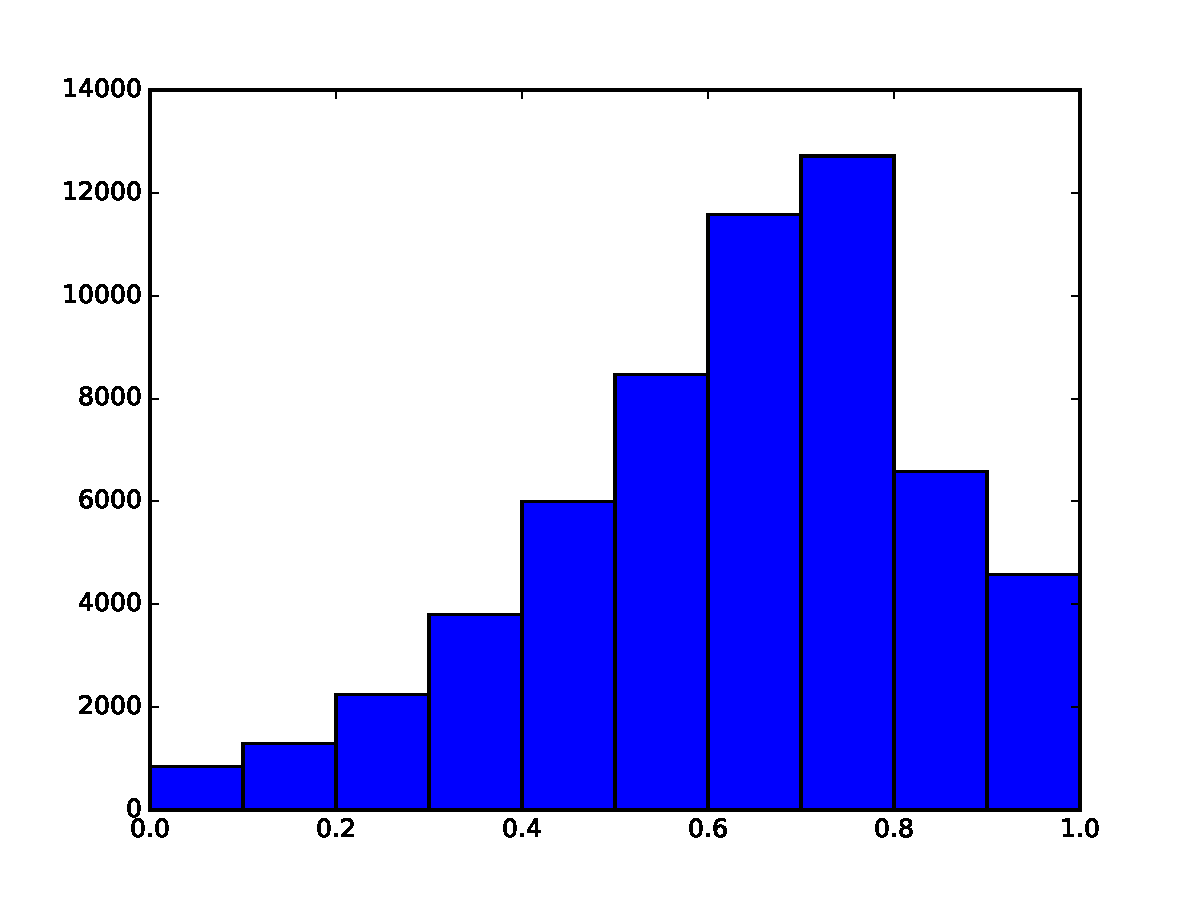
\includegraphics[width=7.5cm]{../secondNet/cosine_same.pdf}
    \label{cos_same}
    \caption{Repartition of the cosine distance between deep vectors from the same speaker}
\end{figure}
\begin{figure}[!h]
    \centering
    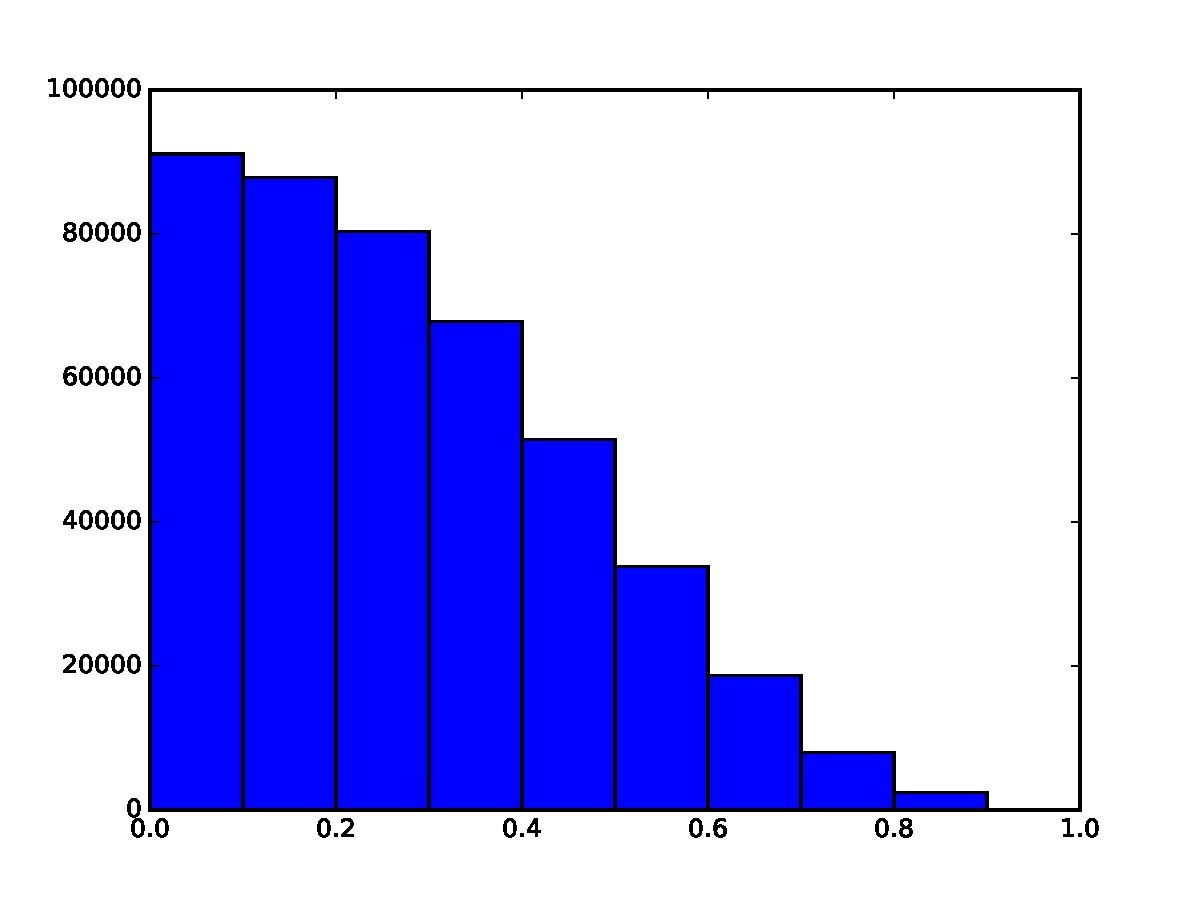
\includegraphics[width=7.5cm]{../secondNet/cosine_diff.pdf}
	\label{cos_diff}    
    \caption{Repartition of the cosine distance between deep vectors from different speakers}
\end{figure}

\begin{figure}[!h]
    \centering
    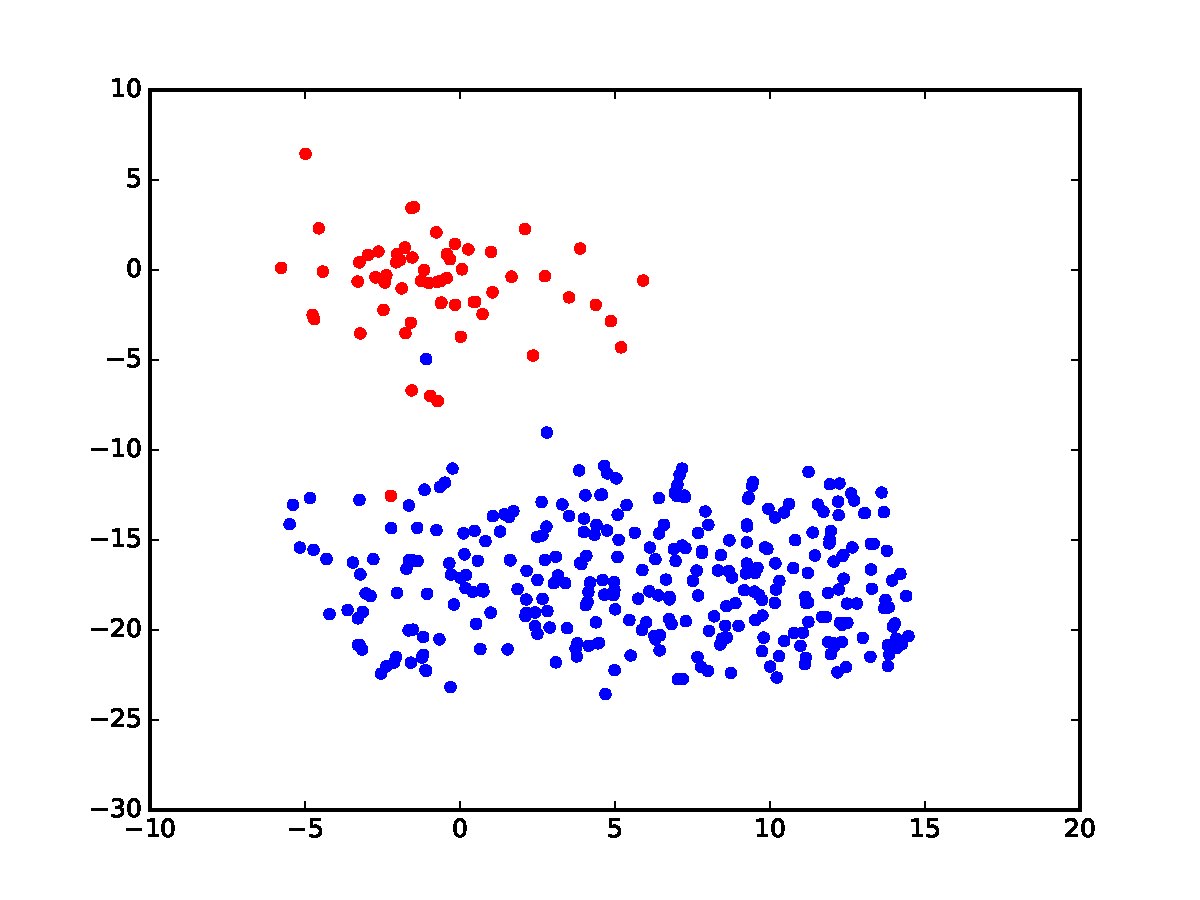
\includegraphics[width=7.5cm]{../secondNet/tSNE_HOUDIN_TRUCHOT.pdf}
	\label{tSNE}
    \caption{t-SNE of the deep vectors of two different speakers}
\end{figure}


Figure \ref{tSNE} also encourages us to believe that the deep vectors will provide a good separabiliy. In fact, t-Distributed Stochastic Neighbor Embedding (t-SNE) provides a reduction of the vectors in a 2 dimensions space in order to have a good visualization of high dimensional data \cite{ictdbid:2777}.

We ran many experiments and therefore cannot present them all. We will only present the most interesting. The configuration and DET graphs of our experiments are presented in the annex.

\section{Further work}


\newpage
\printbibliography

\newpage

\appendix

%Experiment 0
\begin{table}[!h]
\centering
\begin{tabular}{|l|c|c|c|c|c|}
\hline
Number of layers & \multicolumn{5}{c|}{5}                \\ \hline
Size of layers   & 2304   & 1000   & 50  & 1000  & 2304  \\ \hline
Tied weights     & \multicolumn{5}{c|}{No}               \\ \hline
Optimizer        & \multicolumn{5}{c|}{Gradient Descent} \\ \hline
Dropout          & \multicolumn{5}{c|}{0.90} \\ \hline
\end{tabular}
\end{table}

\begin{figure}[!h]
    \centering
    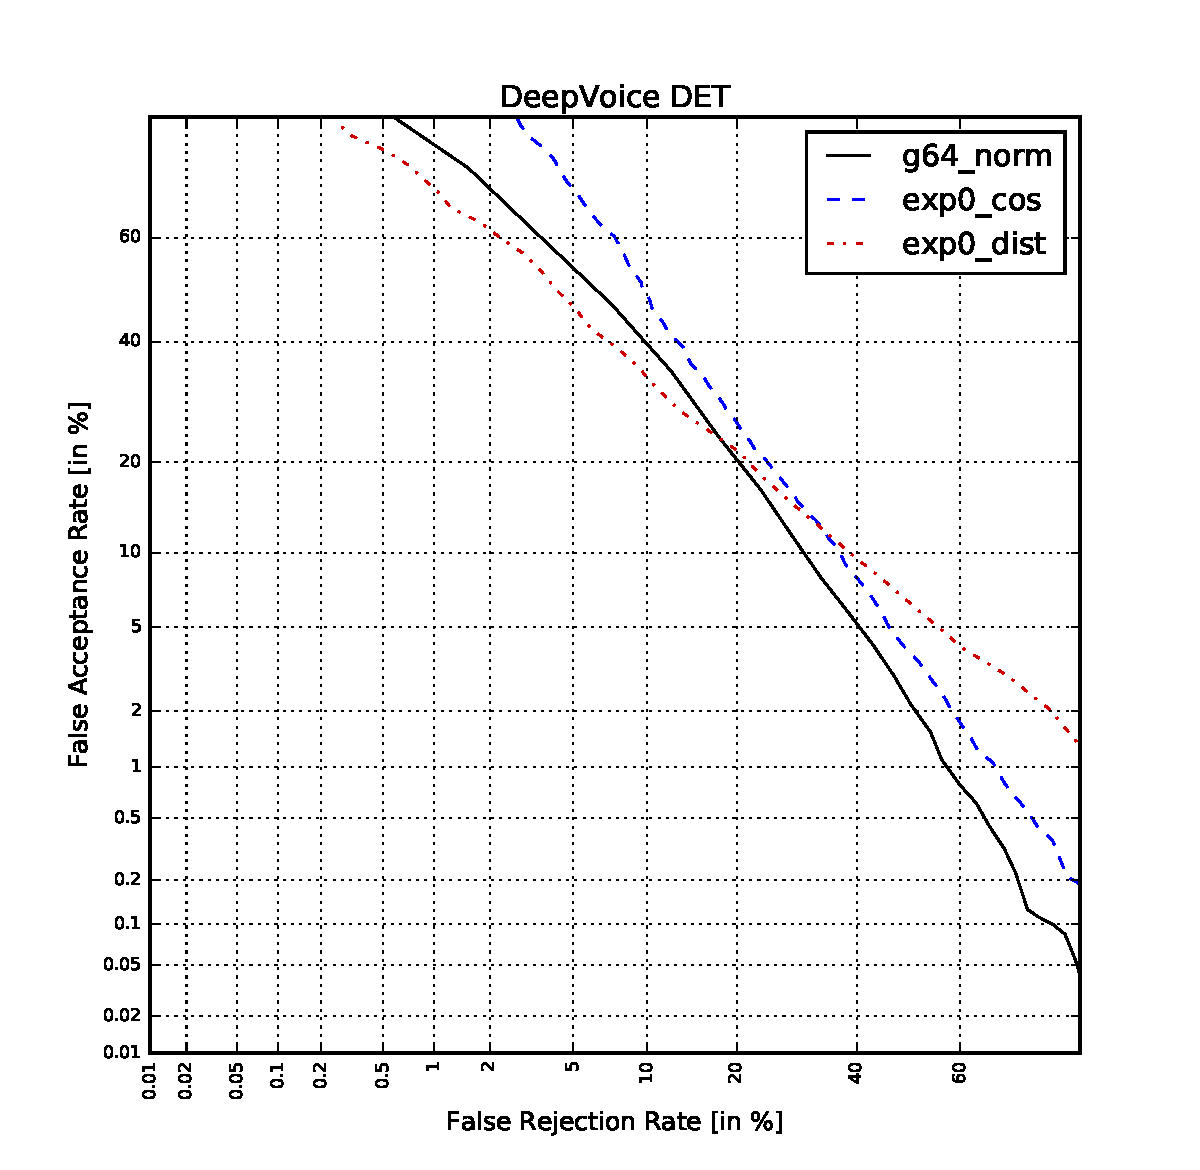
\includegraphics[width=7.5cm]{../scores/det0.pdf}
    \captionsetup{labelformat=empty}
    \caption{Experiment 0}
\end{figure}

\hrule
\vspace{0.5cm}

%Experiment 1
\begin{table}[!h]
\centering
\begin{tabular}{|l|c|c|c|c|c|}
\hline
Number of layers & \multicolumn{5}{c|}{5}                \\ \hline
Size of layers   & 2304   & 1000   & 50  & 1000  & 2304  \\ \hline
Tied weights     & \multicolumn{5}{c|}{No}               \\ \hline
Optimizer        & \multicolumn{5}{c|}{Adam} \\ \hline
Dropout          & \multicolumn{5}{c|}{0.90} \\ \hline
\end{tabular}
\end{table}

\begin{figure}[!h]
    \centering
    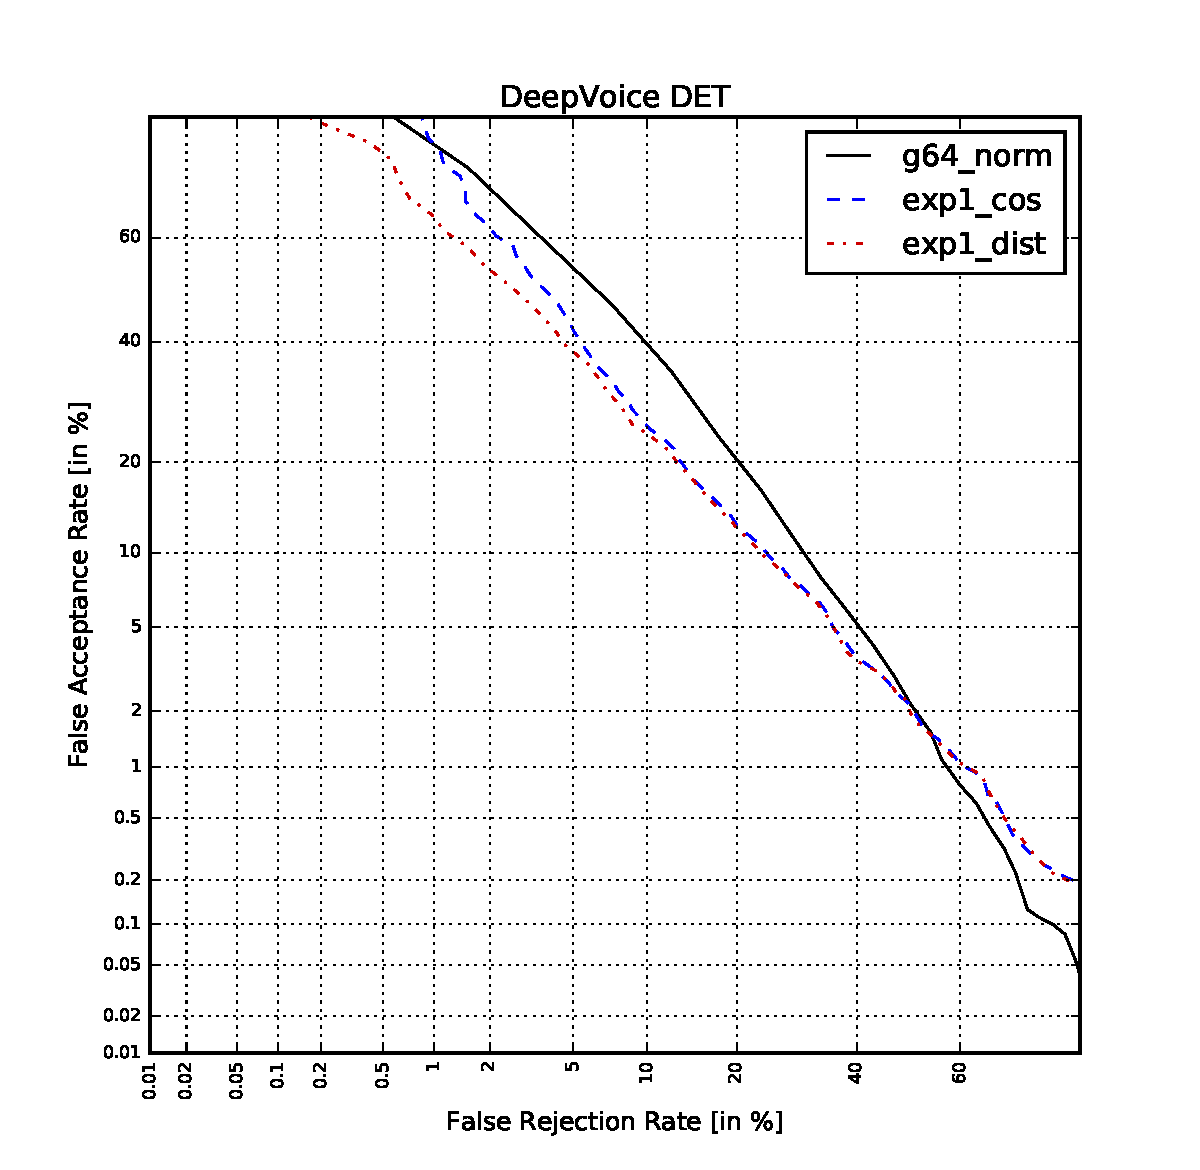
\includegraphics[width=7.5cm]{../scores/det1.pdf}
    \captionsetup{labelformat=empty}
    \caption{Experiment 1}
\end{figure}


\newpage

%Experiment 2
\begin{table}[!h]
\centering
\begin{tabular}{|l|c|c|c|c|c|}
\hline
Number of layers & \multicolumn{5}{c|}{5}                \\ \hline
Size of layers   & 2304   & 480   & 100  & 480  & 2304   \\ \hline
Tied weights     & \multicolumn{5}{c|}{No}               \\ \hline
Optimizer        & \multicolumn{5}{c|}{Adam} \\ \hline
Dropout          & \multicolumn{5}{c|}{0.90} \\ \hline
\end{tabular}
\end{table}


\begin{figure}[!h]
    \centering
    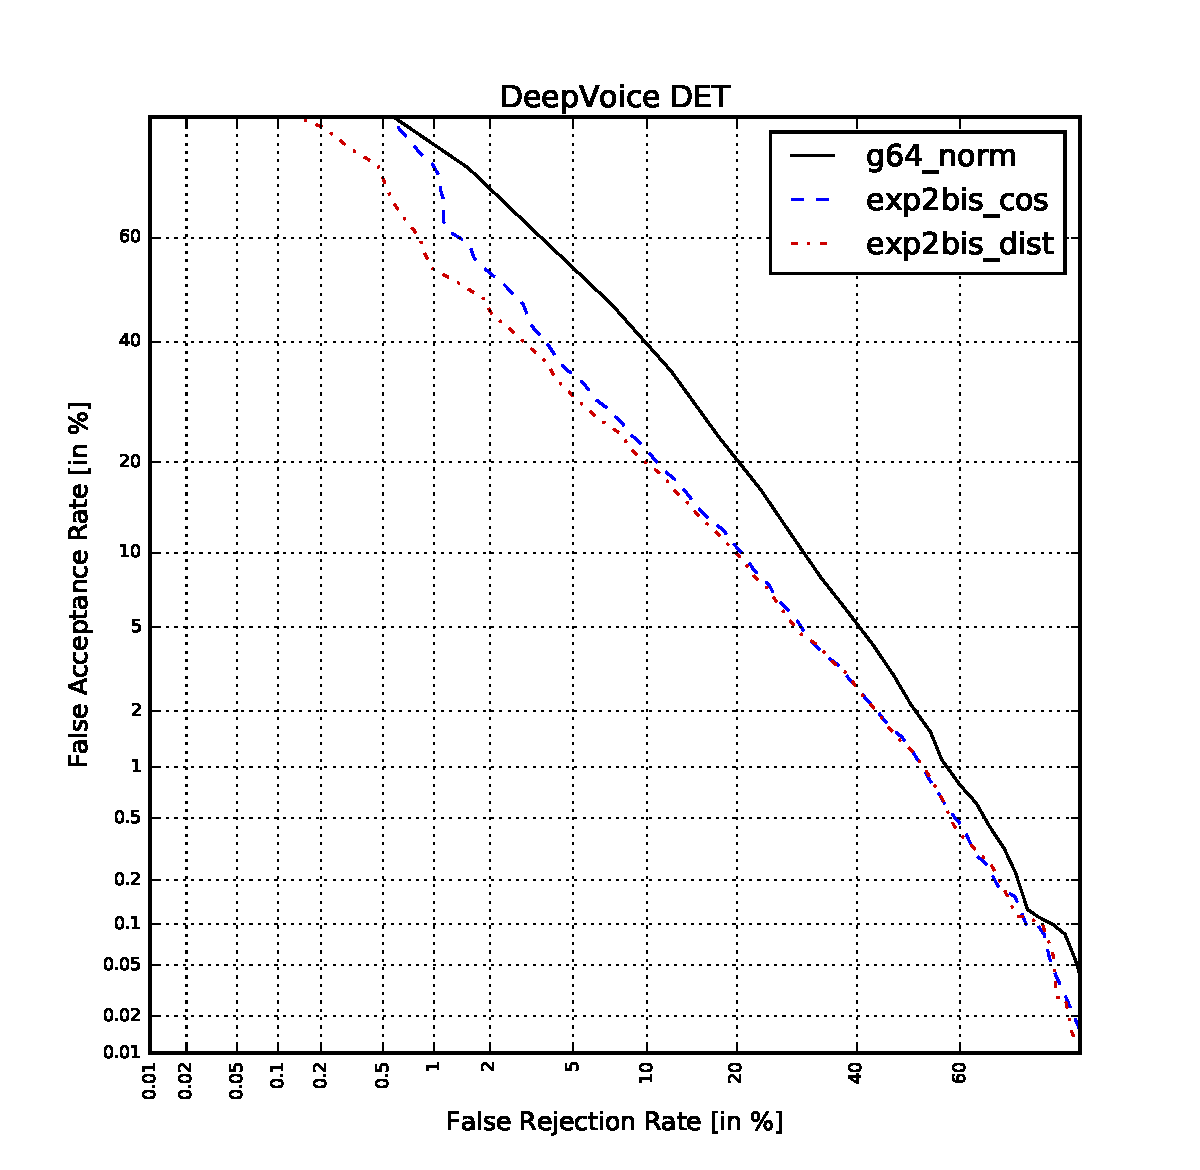
\includegraphics[width=7.5cm]{../scores/det2bis.pdf}
    \captionsetup{labelformat=empty}
    \caption{Experiment 2}
\end{figure}

\hrule
\vspace{0.5cm}

%Experiment 3
\begin{table}[!h]
\centering
\begin{tabular}{|l|c|c|c|c|c|c|c|}
\hline
Number of layers & \multicolumn{7}{c|}{7}                \\ \hline
Size of layers   & 2304 & 720 & 225 & 70 & 225 & 720 & 2304  \\ \hline
Tied weights     & \multicolumn{7}{c|}{No}               \\ \hline
Optimizer        & \multicolumn{7}{c|}{Adam} \\ \hline
Dropout          & \multicolumn{7}{c|}{0.90} \\ \hline
\end{tabular}
\end{table}

\begin{figure}[!h]
    \centering
    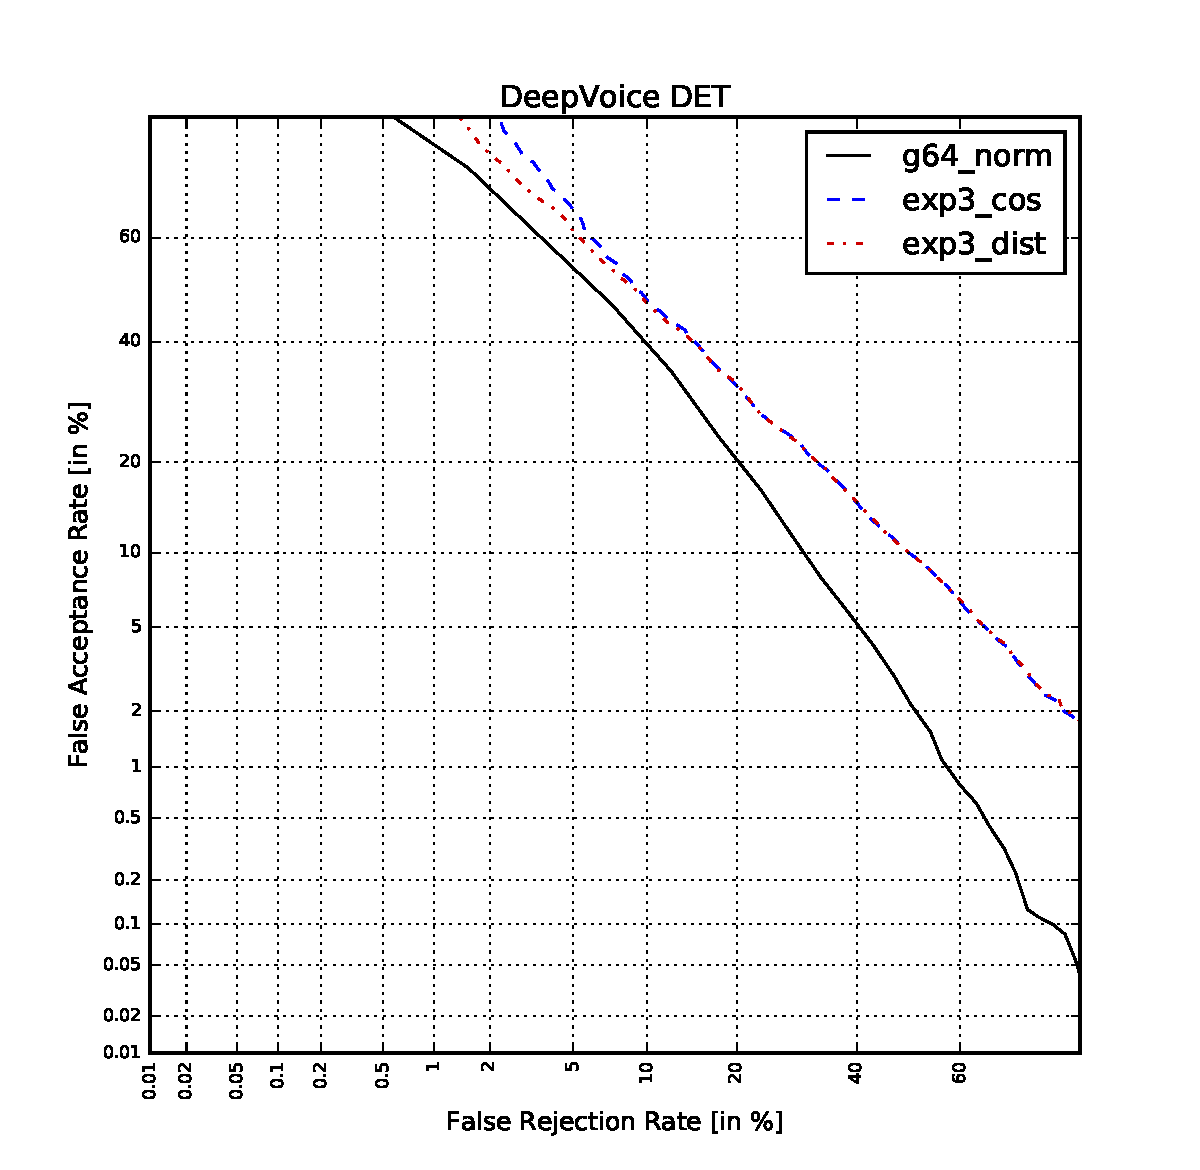
\includegraphics[width=7.5cm]{../scores/det3.pdf}
    \captionsetup{labelformat=empty}
    \caption{Experiment 3}
\end{figure}


\newpage

%Experiment 4
\begin{table}[!h]
\centering
\begin{tabular}{|l|c|c|c|c|c|c|c|}
\hline
Number of layers & \multicolumn{7}{c|}{7}                \\ \hline
Size of layers   & 2304 & 720 & 225 & 70 & 225 & 720 & 2304  \\ \hline
Tied weights     & \multicolumn{7}{c|}{Yes}               \\ \hline
Optimizer        & \multicolumn{7}{c|}{Adam} \\ \hline
Dropout          & \multicolumn{7}{c|}{0.90} \\ \hline
\end{tabular}
\end{table}


\begin{figure}[!h]
    \centering
    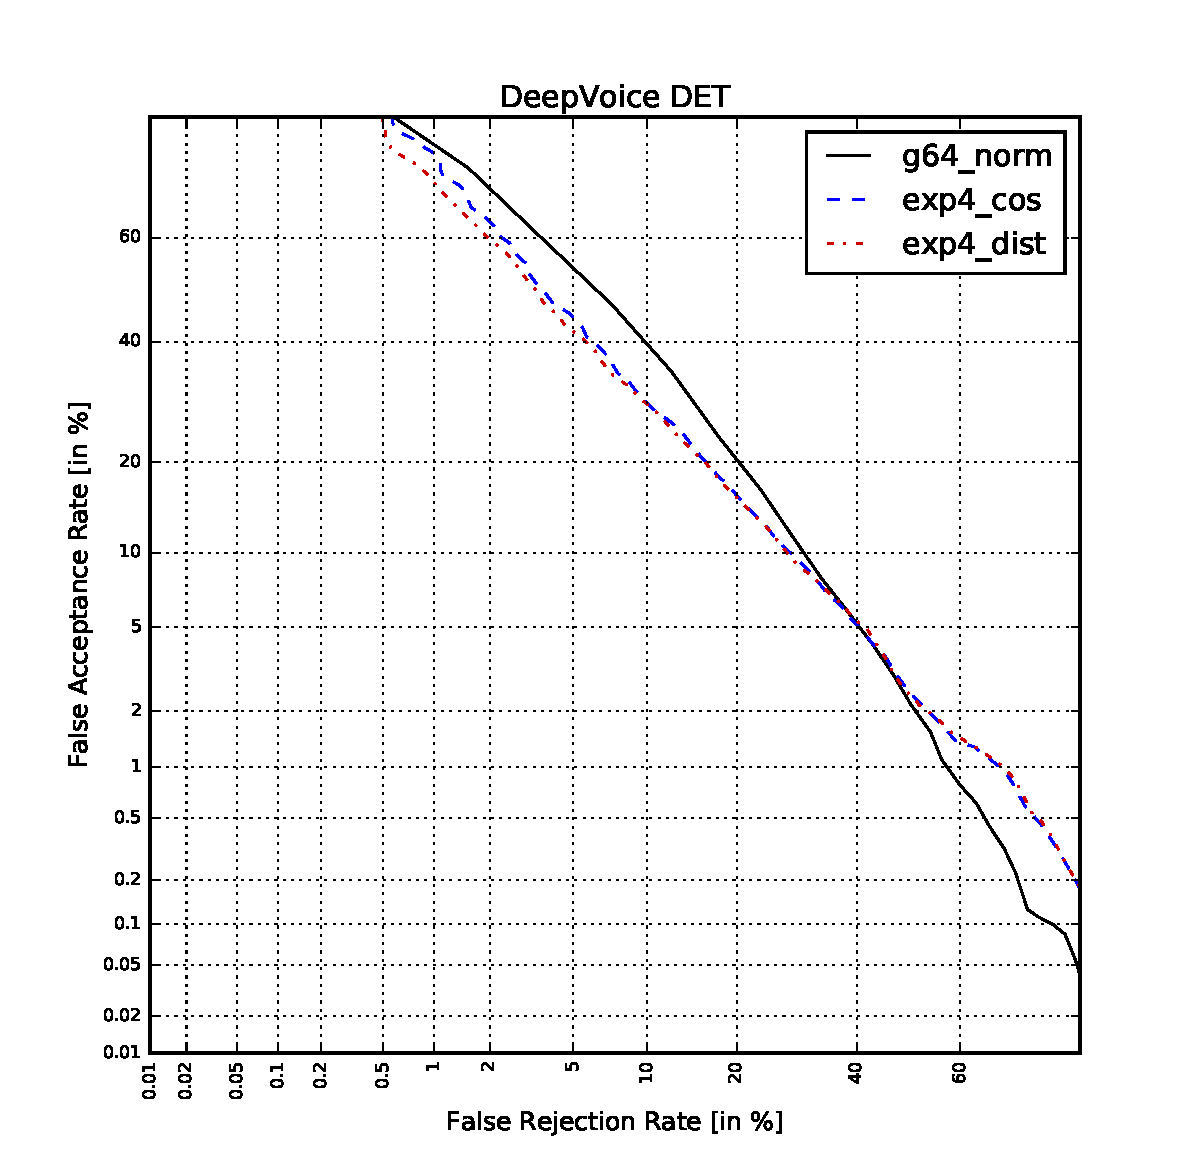
\includegraphics[width=7.5cm]{../scores/det4.pdf}
    \captionsetup{labelformat=empty}
    \caption{Experiment 4}
\end{figure}

\hrule
\vspace{0.5cm}


%Experiment 5
%\begin{table}[!h]
%\centering
%\begin{tabular}{|l|c|c|c|c|c|c|c|}
%\hline
%Number of layers & \multicolumn{7}{c|}{7}                \\ \hline
%Size of layers   & 2304 & 1000 & 300 & 60 & 300 & 1000 & 2304  \\ \hline
%Tied weights     & \multicolumn{7}{c|}{Yes}               \\ \hline
%Optimizer        & \multicolumn{7}{c|}{Adam} \\ \hline
%Dropout          & \multicolumn{7}{c|}{0.90} \\ \hline
%\end{tabular}
%\end{table}

%\begin{figure}[!h]
%    \centering
%    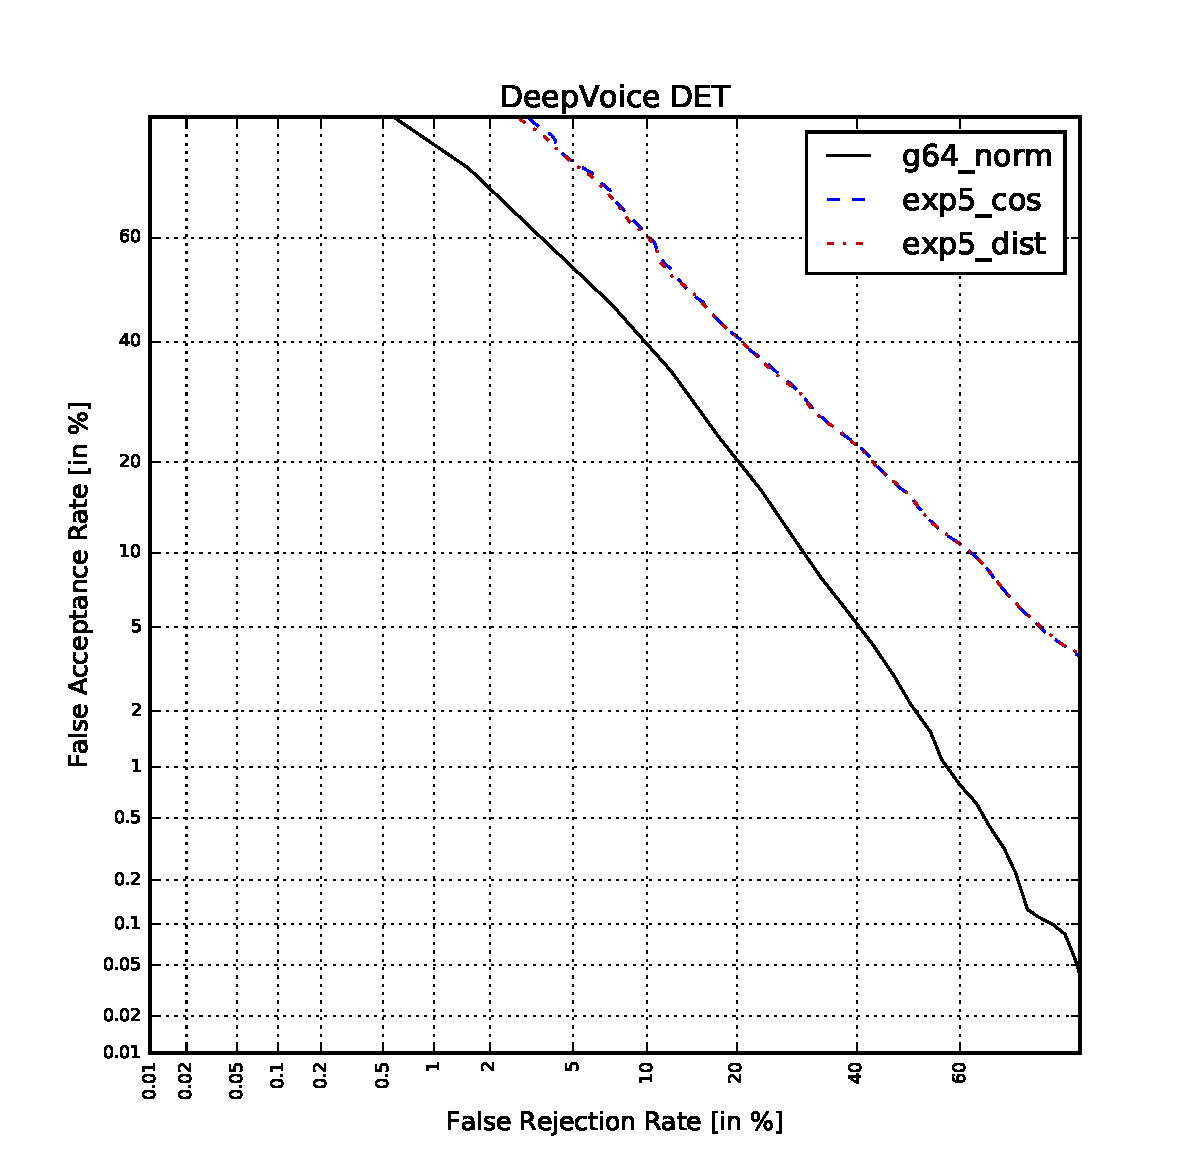
\includegraphics[width=7.5cm]{../scores/det5.pdf}
%    \caption{Experiment 5}
%\end{figure}


%\newpage


%Experiment 7
\begin{table}[!h]
\centering
\begin{tabular}{|l|c|c|c|c|c|}
\hline
Number of layers & \multicolumn{5}{c|}{5}                \\ \hline
Size of layers   & 2304   & 500   & 80  & 500  & 2304   \\ \hline
Tied weights     & \multicolumn{5}{c|}{No}               \\ \hline
Optimizer        & \multicolumn{5}{c|}{Adam} \\ \hline
Dropout          & \multicolumn{5}{c|}{0.80} \\ \hline
\end{tabular}
\end{table}


\begin{figure}[!h]
    \centering
    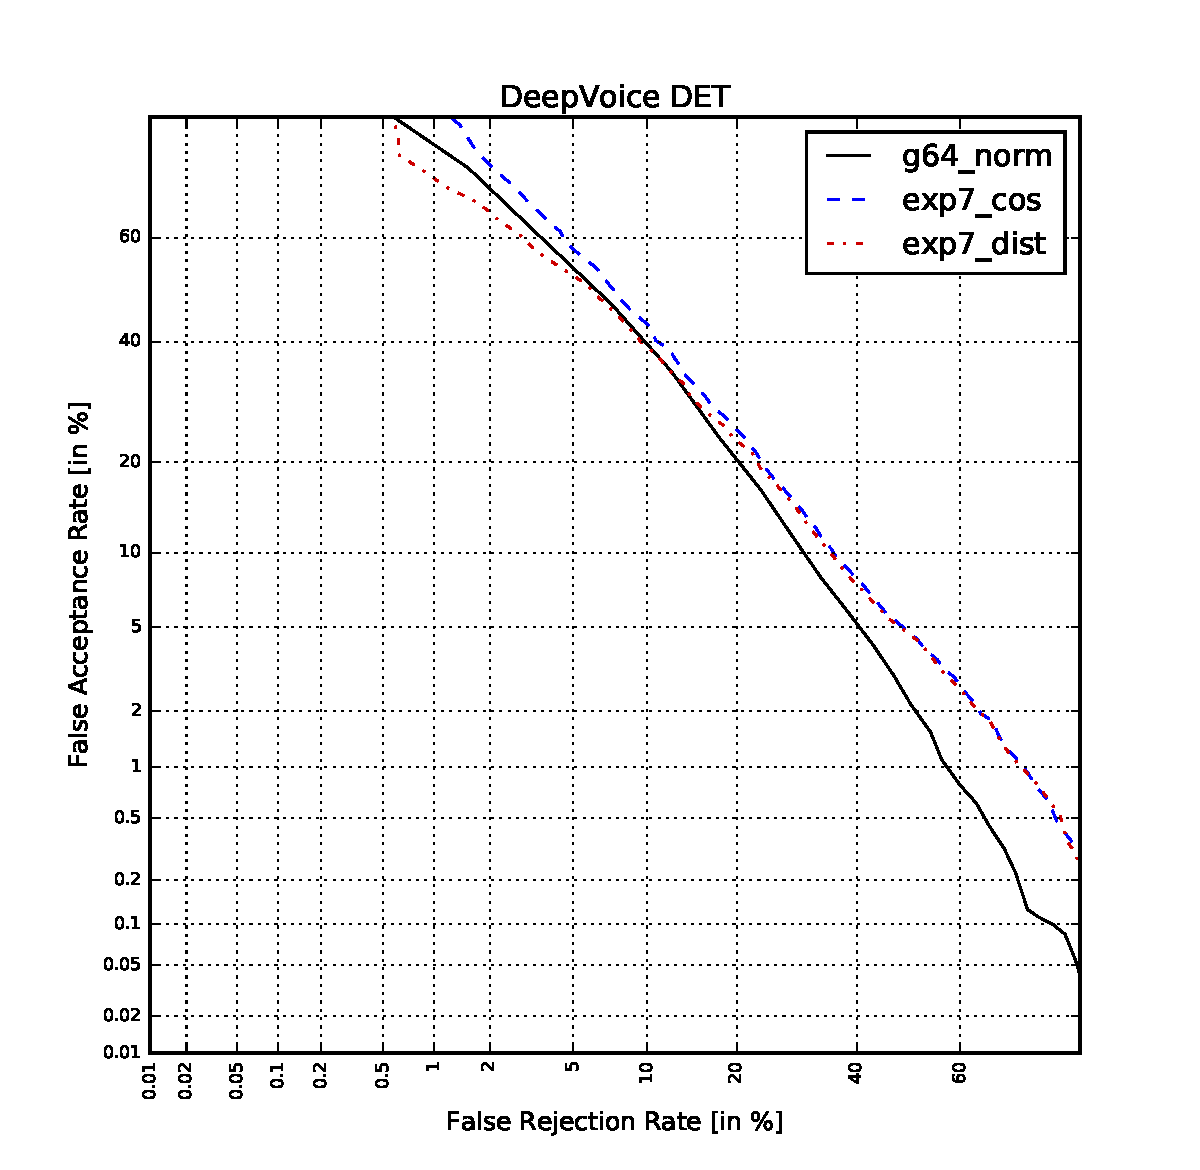
\includegraphics[width=7.5cm]{../scores/det7.pdf}
    \captionsetup{labelformat=empty}
    \caption{Experiment 7}
\end{figure}






\end{document}
